\section{ỨNG DỤNG HỆ PHƯƠNG TRÌNH BẬC NHẤT BA ẨN}
\subsection{Các dạng toán và ví dụ}
\begin{dang}{Giải bài toán bằng cách lập hệ phương trình}
	Để giải bài toán bằng cách lập hệ phương trình bậc nhất ba ẩn, ta thực hiện các bước sau:\\
	\textbf{Bước 1: }Lập hệ phương trình.\\
	Chọn ẩn là những đại lượng chưa biết.\\
	Dựa trên ý nghĩa của các đại lượng chưa biết, đặt điều kiện cho ẩn.\\
	Dựa vào dữ kiện của bài toán, lập hệ phương trình với các ẩn.\\
	\textbf{Bước 2:} Giải hệ phương trình.\\
	\textbf{Bước 3: }Kiểm tra điều kiện của nghiệm và kết luận.
	\end{dang}
\begin{vd}%[0D3B3-5]
	Một cửa hàng bán áo sơ mi, quần nam và váy nữ. Ngày thứ nhất bán được $21$ áo, $21$ quần và $18$ váy, doanh thu là $5349000$ đồng. Ngày thứ hai bán được $16$ áo, $24$ quần và $12$ váy, doanh thu là $5600000$ đồng. Ngày thứ ba bán được $24$ áo, $15$ quần và $12$ váy, doanh thu là $5259000$ đồng. Khi đó giá bán mỗi áo, mỗi quần và mỗi váy bằng bao nhiêu?	\loigiai
	{		Gọi giá tiền mỗi chiếc áo, quần và váy lần lượt là $x$, $y$, $z$ \big(đồng, $ x$, $y$, $z > 0$\big) \\
		Theo đề bài ta có hệ phương trình $ \heva{& 21x + 21y + 18z = 5349000 \\ & 16x + 24y + 12z = 5600000 \\ & 24x + 15y + 12z = 5259000 } \Leftrightarrow \heva{& x = 98000 \\ & y = 125000 \\ & z = 86000.} $ \\
		Vậy giá tiền mỗi chiếc áo, quần và váy lần lượt là $ 98000$, $125000$, $86000 $ \big(đồng\big).
	}
\end{vd}
\begin{vd}%[0D3B3-5]
	Ba cô Lan, Hương và Thúy cùng thêu một loại áo giống nhau. Số áo của Lan thêu trong $1$ giờ ít hơn tổng số áo của Hương và Thúy thêu trong $1$ giờ là $5$ áo. Tổng số áo của Lan thêu trong $4$ giờ và Hương thêu trong $3$ giờ nhiều hơn số áo của Thúy thêu trong $5$ giờ là $30$ áo. Số áo của Lan thêu trong $2$ giờ cộng với số áo của Hương thêu trong $5$ giờ và số áo của Thúy thêu trong $3$ giờ tất cả được $76$ áo. Hỏi trong $1$ giờ mỗi cô thêu được mấy áo?
	\loigiai{
		Gọi $ x, y, x $	lần lượt là số áo của Lan, Hương, Thúy thêu được trong $ 1 $ giờ. Điều kiện là $ x, y, z \in \mathbb{N^*} $. \\
		Theo đề bài ta có hệ phương trình: $$ \heva{& x = y + z -5 \\& 4x + 3y - 5z = 30 \\& 2x + 5y + 3z =76} \Leftrightarrow \heva{& x - y - z = 5 \\& 4x + 3y - 5z = 30 \\& 2x + 5y + 3z =76} \Leftrightarrow \heva{& x = 9 \\& y = 8 \\& z = 6.}$$ 
		Vậy trong $1$ giờ Lan thêu được $9$ áo, Hương thêu được $8$ áo, Thúy thêu được  $6$ áo.
	}
\end{vd}
\begin{vd}%[0D3B3-5]
	Ba phân số đều có tử số là $1$ và tổng của ba phân số đó bằng $1$. Hiệu của phân số thứ nhất và phân số thứ hai bằng phân số thứ ba, còn tổng của phân số thứ nhất và phân số thứ hai bằng $5$ lần phân số thứ ba. Khi đó tích ba phân số đó bằng bao nhiêu?
	\loigiai
	{
		Gọi ba phân số lần lượt là $ \dfrac{1}{x}$, $\dfrac{1}{y}$, $\dfrac{1}{z}$. \\
		Theo đề bài ta có hệ phương trình: $$\heva{& \dfrac{1}{x} + \dfrac{1}{y} + \dfrac{1}{z} = 1 \\ & \dfrac{1}{x} - \dfrac{1}{y} = \dfrac{1}{z} \\ & \dfrac{1}{x} + \dfrac{1}{y} = \dfrac{5}{z}} \Leftrightarrow \heva{& \dfrac{1}{x} = \dfrac{1}{2} \\ & \dfrac{1}{y} = \dfrac{1}{3} \\ & \dfrac{1}{z} =\dfrac{1}{6}.} $$ 
		Vậy $ \dfrac{1}{x} \cdot \dfrac{1}{y} \cdot \dfrac{1}{z} = \dfrac{1}{36}$.
	}
\end{vd}
\begin{dang}{Ứng dụng trong giải bài toán Vật Lý, Hóa Học, Sinh Học.}
	
	\end{dang}
\begin{vd}%[0D3B3-5]
\immini{Cho mạch điện như hình vẽ. Điện trở $R_1=200 \Omega$; hiệu điện thế giữa hai điểm $A$ và $B$ giữ không đổi là $U_{AB}=6 \mathrm{~V}$. Điện trở của ampe kế bằng không, vôn kế có điện trở hữu hạn $R_V$ chưa biết. Số chỉ ampe kế là $10 \mathrm{~mA}$, số chỉ của vôn kế là $4{,}5 \mathrm{~V}$. Tìm giá trị điện trở $R_2$ và điện trở của vôn kế $R_V$?(chiều dòng điện qua ampe kế từ $C$ đến $D$)}{
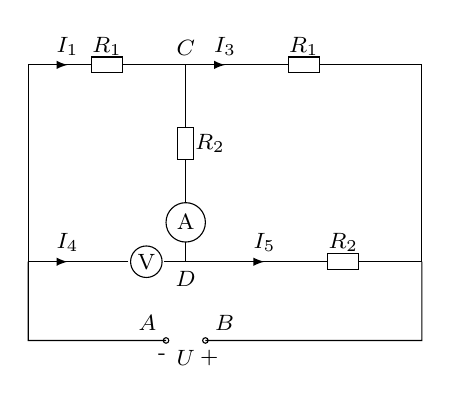
\begin{tikzpicture}
	\tikzset{
		every node/.style={font=\footnotesize,transform shape},
		%
		ampe/.pic={\draw (0,0)circle(0.25) (0,0)node[align=center]{A};},
		%
		vol/.pic={\draw (0,0)circle(0.2) (0,0)node[align=center]{V};},
		% Điện tro
		dientro2/.pic={\draw (-.1,-.2)--(-.1,.2)--(.1,.2)--(.1,-.2)--cycle %(0,0)node[align=center]{Hình\\chữ nhật}
			;},
		% Điện tro
		dientro/.pic={\draw (-.2,-.1)--(-.2,.1)--(.2,.1)--(.2,-.1)--cycle %(0,0)node[align=center]{Hình\\chữ nhật}
			;},
		% Điện tro
		dientro1/.pic={\draw (-.2,-.1)--(-.2,.1)--(.2,.1)--(.2,-.1)--cycle %(0,0)node[align=center]{Hình\\chữ nhật}
			;},
		% Điện tro
		dientro3/.pic={\draw (-.2,-.1)--(-.2,.1)--(.2,.1)--(.2,-.1)--cycle %(0,0)node[align=center]{Hình\\chữ nhật}
			;},
	}
	%
	\draw
	(0,0)pic[local bounding box =am]{ampe}
	(2,-.5)pic[local bounding box =dt3]{dientro3}
	(-1,2)pic[local bounding box =dt]{dientro}
	(1.5,2)pic[local bounding box =dt1]{dientro1}
	(0,1)pic[local bounding box =dt2]{dientro2}
	(-.5,-.5)pic[local bounding box =vol]{vol}
	;
	%
	\draw[](0,-.5)--(am)--(dt2)node[right]{$R_2$}--(0,2)node[above]{$C$}--(dt1)--(3,2)--(3,-.5)--(dt3)node[above]{$R_2$}--(0,-.5)node[below]{$D$}--(vol)--(-2,-.5)--(-2,2)--(dt)node[above]{$R_1$}--(0,2);
	\draw[-latex](0,2)--(0.5,2)node[above]{$I_3$};
	\draw[-latex](-2,-.5)--(-1.5,-.5)node[above]{$I_4$};
	\draw[-latex](-2,2)--(-1.5,2)node[above]{$I_1$};
	\draw[-latex](0.5,-.5)--(1,-.5)node[above]{$I_5$};
	\draw(-2,-.5)--(-2,-1.5)--(-.25,-1.5)node[above left]{$A$}circle(1pt) (.25,-1.5)node[above right]{$B$}circle(1pt)--(3,-1.5)--(3,-.5) (0,-1.5)node[below]{$U$} (0.3,-1.5)node[below]{+} (-0.3,-1.5)node[below]{-} (dt1)node[above]{$R_1$};
\end{tikzpicture}
}
\loigiai{Ta có $	U_{D B}=U-U_{A D}=1{,}5 \mathrm{~V}$.\\
	Do dòng điện đi theo chiều từ $C$ tới $D$
	$$
	\begin{aligned}
		U_{A D} &=U_{A C}+U_{C D} \\
		U_{A D} &=I_1 R_1+I_2 R_2 \\
		4{,}5=& I_1 \cdot 200+0{,}01 \cdot R_2 \quad(1)
			\end{aligned}$$
và $$			\begin{aligned}
		& U_{D B}=U_{D C}+U_{C B} \\
		& U_{D B}=-I_2 R_2+I_3 R_1 \\
		& 1,5=0,01 \cdot R_2+I_3 \cdot 200\quad(2)
	\end{aligned}
	$$
	Tại nút $C$ có:
	$	I_1=I_2+I_3=0{,}01+I_3$.\quad(3)\\
Từ  (1), (2), (3) có hệ ba phương trình ba ẩn $I_1$, $I_3$, $R_2$
	$$
	\left\{\begin{array} { l } 
		{ 4 , 5 = I _ { 1 } \cdot 2 0 0 + 0 , 0 1 \cdot R _ { 2 } } \\
		{ 1 , 5 = 0 , 0 1 \cdot R _ { 2 } + I _ { 3 } \cdot 2 0 0 } \\
		{ I _ { 1 } = I _ { 2 } + I _ { 3 } = 0 , 0 1 + I _ { 3 } }
	\end{array} \Leftrightarrow \left\{\begin{array}{l}
		I_1=0{,}02 \mathrm{~A} \\
		I_3=0{,}01 \mathrm{~A} \\
		R_2=50 \Omega.
	\end{array}\right.\right.
	$$
Vậy $I_5=\dfrac{U_{D B}}{R_2}=\dfrac{1{,}5}{50}=0{,}03 \mathrm{~A}$; $I_4=I_5-I_2=0{,}02 \mathrm{~A}$;
		$ R_V=\dfrac{U_{A D}}{I_4}=\dfrac{4{,}5}{0{,}02}=250 \Omega$.
}
	\end{vd}
\begin{vd}%[0D3B3-5]
	Cân bằng phương trình sau
$\mathrm{CH}_4+\mathrm{O}_2\rightarrow\mathrm{CO}_2+\mathrm{H}_2 \mathrm{O}$.
\loigiai{
Để cân bằng phản ứng, ta cần tìm các số nguyên dương $x, y, z, t$ sao cho $$x \mathrm{CH}_4+\mathrm{yO}_2\rightarrow\mathrm{zCO}_2+\mathrm{tH}_2 \mathrm{O}.$$
Đối với mỗi nguyên tố, số nguyên tử ở vế phải và vế trái phải bằng nhau, ta có\\
Carbon: $x=z$;
Hydrogen: $4 x=2 t$;
Oxygen: $2 y=2 z+t$.\\
Từ đó ta có hệ phương trình:
$\heva{&x-z=0\\&4 x-2 t=0\\&2 y-2 z-t=0.}$\\
Giải hệ, ta có nghiệm tổng quát
$x=\dfrac{t}{2}$, $y=t$, $z=\dfrac t2$, với $t$ là số thực tùy ý.\\
Số nguyên dương $t$ nhỏ nhất để $x, y, z, t$ là nguyên dương là $t=2$.\\
Do đó cân bằng được phương trình phản ứng:
$\mathrm{CH}_4+2 \mathrm{O}_2\rightarrow\mathrm{CO}_2+2 \mathrm{H}_2 \mathrm{O}$.
}
	\end{vd}
\begin{vd}%[0D3B3-5]
	Cần 3 thành phần khác nhau $\mathrm{A}, \mathrm{B}$ và $\mathrm{C}$, để sản xuất một lượng hợp chất hóa học nào đó. $\mathrm{A}, \mathrm{B}$ và C phải được hòa tan trong nước một cách riêng biệt trước khi chúng kết hợp lại để tạo ra hợp chất hóa học. Biết rằng nếu kết hợp dung dịch chứa $\mathrm{A}$ với tỉ lệ $1{,}5 \mathrm{~g} / \mathrm{cm}$ với dung dịch chứa $\mathrm{B}$ với tỉ lệ $3{,}6 \mathrm{~g} / \mathrm{cm}$ và dung dịch chứa $\mathrm{C}$ với tỉ lệ $5{,}3 \mathrm{~g} / \mathrm{cm}$ thì tạo ra $25{,}07 \mathrm{~g}$ hợp chất hóa học đó. Nếu tỉ lệ của $\mathrm{A}, \mathrm{B}, \mathrm{C}$ trong phương án này thay đổi thành tương ứng $2{,}5$; $4{,}3$ và $2{,}4 \mathrm{~g} / \mathrm{cm}$ (trong khi thể tích là giống nhau), khi đó $22{,}36 \mathrm{~g}$ chất hóa học sẽ được tạo ra. Cuối cùng, nếu tỉ lệ tương ứng là $2{,}7$; $5{,}5$ và $3{,}2 \mathrm{~g} / \mathrm{cm}$, thì sẽ tạo ra $28{,}14 \mathrm{~g}$ hợp chất. Thể tích của dung dịch chứa $\mathrm{A}$, $\mathrm{B}$ và $\mathrm{C}$ là bao nhiêu?
\loigiai{
	Gọi $x$, $y$, $z$ tương ứng là thể tích $(\mathrm{cm})$ của phương án chứa $\mathrm{A}$, $\mathrm{B}$ và $\mathrm{C}$. \\
	Khi đó $1{,}5x$ là khối lượng của $\mathrm{A}$ trong trường hợp đầu, $3{,}6y$ là khối lượng của $\mathrm{B}$ và $5{,}3 z$ là khối lượng của $\mathrm{C}$.\\
	 Cộng lại với nhau, ba khối lượng này sẽ tạo ra $25{,}07$ g.\\
	 Do đó: $1{,}5 x+3{,}6 y+5{,}32=25{,}07$.\\
	Tương tự cho hai trường hợp còn lại, ta có hệ phương trình :
	$$
	\left\{\begin{array}{l}
		1{,}5 x+3{,}6 y+5{,}32=25{,}07 \\
		2{,}5 x+4{,}3 y+2{,}4 z=22{,}36 \\
		2{,}7 x+5{,}5 y+3{,}22=28{,}14.
	\end{array}\right.
	$$
	Giải hệ trên cho ta nghiệm là $x=1{,}5$; $y=3{,}1$; $z=2{,}2$.
	}
	\end{vd}
\begin{dang}{Ứng dụng trong giải bài toán kinh tế}
	
	\end{dang}
\begin{vd}%[0D3B3-5]
	Xét thị trường chè, cà phê và ca cao. Gọi $x, y$ và $z$ lần lượt là giá của $1 \mathrm{~kg}$ chè, $1 \mathrm{~kg}$ cà phê và $1 \mathrm{~kg}$ ca cao (đơn vị: nghìn đồng, $x \geq 0$, $y \geq 0$, $z \geq 0$ ). Các lượng cung và lượng cầu của mỗi sản phẩm được cho như bảng sau:\begin{center}
	\begin{tabular}{|l|c|c|}
		\hline \multicolumn{1}{|c|}{ Sản phẩm } & Lượng cung & Lượng cầuu \\
		\hline Chè & $Q_{S_1}=-380+x+y$ & $Q_{D_1}=350-x-z$ \\
		\hline Cà phê & $Q_{S_2}=-405+x+2 y-z$ & $Q_{D_2}=760-2 y-z$ \\
		\hline Ca cao & $Q_{S_3}=-350-2 x+3 z$ & $Q_{D_3}=145-x+y-z$ \\
		\hline
	\end{tabular}
\end{center}
	Tìm giá của mỗi kilôgam chè, cà phê và ca cao để thị trường cân bằng.
	\loigiai{
Thị trường cân bằng khi $\left\{\begin{array}{l}Q_{S_1}=Q_{D_1} \\ Q_{S_2}=Q_{D_2} \\ Q_{S_3}=Q_{D_3}\end{array}\right.$ hay $\left\{\begin{array}{l}2 x+y+z=730 \\ x+4 y=1165 \\ -x-y+4 z=495.\end{array}\right.$.\\
Giải hệ phương trình, ta được: $x=125, y=260, z=220$.\\
Vậy giá của mỗi kilôgam chè, cà phê, ca cao lần lượt là 125000 đồng, 260000 đồng, 220000 đồng.	
}
	\end{vd}
\begin{vd}%[0D3B3-5]
	Một đoàn xe tải chở $290$ tấn xi măng cho một công trình xây đập thuỷ điện. Đoàn xe có $57$ chiếc gồm ba loại, xe chở 3 tấn, xe chở 5 tấn và xe chở $7{,}5$ tấn. Nếu dùng tất cả xe $7{,}5$ tấn chở ba chuyến thì được số xi măng bằng tổng số xi măng do xe 5 tấn chở ba chuyến và xe 3 tấn chở hai chuyến. Hỏi số xe mỗi loại?
	\loigiai{
	Gọi $x$ là số xe tải chở 3 tấn, $y$ là số xe tải chở 5 tấn và $z$ là số xe tải chở 7,5 tấn. Điều kiện $x, y, z$ nguyên dương.
	Theo giả thiết của bài toán ta có
	$$
\heva{
		x + y + z & = 5 7  \\
		3 x + 5 y + 7{,}5 z  & = 2 9 0  \\
		2 2 {,}5 z  &  = 6 x + 1 5 y 
	} \Leftrightarrow \heva{
		x+y+z & =57 \\
		3 x+5 y+7{,}5 z & =290 \\
		-2 x-5 y+7{,}5 z & =0.
}	$$
	Giải hệ phương trình ta được $x=20$, $y=19$, $z=18$.\\
	Vậy có $20$ xe chở 3 tấn, $19$ xe chở $5$ tấn, $18$ xe chở $7{,}5$ tấn
}
\end{vd}
\subsection{Bài tập rèn luyện}
%CTST
\begin{bt}%[0D3B3-5]
Ba vận động viên Hùng, Dũng và Mạnh tham gia thi đấu nội dung ba môn phối hợp: chạy, bơi và đạp xe, trong đó tốc độ trung bình của họ trên mỗi chặng đua được cho ở bảng dưới đây.\begin{center}
\begin{tabular}{|c|c|c|c|}
	\hline \multirow{2}{*}{ Vận động viên } & \multicolumn{3}{|c|}{ Tốc độ trung bình (km/h) } \\
	\cline { 2 - 4 } & Chạy & Bơi & Đạp xe \\
	\hline Hùng & $12{,}5$ & $3{,}6$ & $48$ \\
	\hline Dũng & $12$ & $3{,}75$ & $45$ \\
	\hline Mạnh & $12{,}5$ & $4$ & $45$ \\
	\hline
\end{tabular}
\end{center}
Biết tổng thời gian thi đấu ba môn phối hợp của Hùng là $1$ giờ $1$ phút $30$ giây, của Dũng là $1$ giờ $3$ phút $40$ giây và của Mạnh là $1$ giờ $1$ phút $55$ giây. Tính cự li của mỗi chặng đua.
\loigiai{Đổi: $1$ giờ $1$ phút $30$ giây $=\dfrac{41}{40}$ h, $1$ giờ $3$ phút $40$ giây $=\dfrac{191}{180}$ h, $1$ giờ $1$ phút $55$ giây $=\dfrac{743}{720}$ h. Gọi cự li của mỗi chặng đua chạy, bơi và đạp xe lần lượt là $x$, $y$, $z$ (km).\\
	Dựa vào bảng trên ta có hệ phương trình: $\left\{\begin{array}{l}\dfrac{x}{12{,}5}+\dfrac{y}{3{,}6}+\dfrac{z}{48}=\dfrac{41}{40} \\ \dfrac{x}{12}+\dfrac{y}{3{,}75}+\dfrac{z}{45}=\dfrac{191}{180} \\ \dfrac{x}{12{,}5}+\dfrac{y}{4}+\dfrac{z}{45}=\dfrac{743}{720}.\end{array}\right.$\\
	Giải hệ này ta được $x=5$, $y=0{,}75$, $z=20$.\\
	Vậy cự li của mỗi chặng đua chạy, bơi và đạp xe lần lượt là $5$ km; $0{,}75$ km; $20$ km.
}
\end{bt}
\begin{bt}%[0D3B3-5]
	Một nhà hoá học có ba dung dịch cùng một loại acid nhưng với nồng độ khác nhau là $10 \%$, $20 \%$ và $40 \%$. Trong một thí nghiệm, để tạo ra $100 \mathrm{~ml} $ dung dịch nồng độ $18 \%$, nhà hoá học đã sử dụng lượng dung dịch nồng độ $10 \%$ gấp bốn lần lượng dung dịch nồng độ $40 \%$. Tính số mililít dung dịch mỗi loại mà nhà hoá học đó đã sử dụng trong thí nghiệm này.
	\loigiai{Gọi $x$, $y$, $z$ lần lượt là số mililít dung dịch acid có nồng độ $10 \%$, $20 \%$ và $40 \%$ đã sử dụng trong thí nghiệm $(x \geq 0$, $y \geq 0$, $z \geq 0)$.\\
		Theo đề bài, ta có hệ phương trình:
		$\left\{\begin{array}{l}x+y+z=100 \\ x=4 z \\ 0{,}1 x+0{,}2 y+0{,}4 z=0{,}18\cdot100\end{array}\right.$\\
		 hay $\left\{\begin{array}{l}x+y+z=100 \\ x-4 z=0 \\ x+2 y+4 z=180 .\end{array}\right.$\\
		Giải hệ phương trình, ta được $x=40 ; y=50$ và $z=10$.\\
		Vậy lượng acid có nồng độ $10 \%, 20 \%$ và $40 \%$ cần sử dụng lần lượt là $40 \mathrm{~ml}$, $50 \mathrm{~ml}$ và $10 \mathrm{ml}$.
	}
	\end{bt}
\begin{bt}%[0D3B3-5]
	Ba loại tế bào $A$, $B$, $C$ thực hiện số lần nguyên phân lần lượt là $3$, $4$, $7$ và tổng số tế bào con tạo ra là $480$. Biết rằng khi chưa thưc hiện nguyên phân, số tế bào loại $B$ bằng tổng số tế bào loại $A$ và loại $C$. Sau khi thực hiện nguyên phân, tổng số tế bào con loại $A$ và loại $C$ được tạo ra gấp năm lần số tế bào con loại $B$ được tạo ra. Tính số tế bào con mỗi loại lúc ban đầu.
	\loigiai{
	Gọi $x$, $y$, $z$ lần lượt là số tế bào loại $A$, $B$, $C$ lúc ban đầu $(x$, $y$, $z \in \mathbb{N})$.\\
	Ba loại tế bào $A$, $B$, $C$ thực hiện số lần nguyên phân lần lượt là $3$, $4$, $7$ và tổng số tế bào con tạo ra là $480$, ta có $x \cdot 2^3+y \cdot 2^4+z \cdot 2^7=480$ hay $x+2 y+16 z=60$.\\
	Khi chưa thực hiện nguyên phân số tế bào loại $B$ bằng tổng số tế bào loại $A$ và loại $C$, ta có $y=x+z$.\\
	Sau khi thực hiện nguyên phân, tổng số tế bào con loại $A$ và loại $C$ được tạo ra gấp năm lần số tế bào con loại $B$ được tạo ra, ta có $x \cdot 2^3+z \cdot 2^7=5 \cdot y \cdot 2^4$ hay $x+16 z=10 y$.\\
	Từ đó, ta có hệ phương trình
	$$
	\left\{\begin{array}{l}
		x+2 y+16 z=60 \\
		x-y+z=0 \\
		x-10 y+16 z=0.
	\end{array}\right.
	$$
	Giải hệ phương trình, ta được: $x=2$, $y=5$, $z=3$.
	Vậy số tế bào $A$, $B$, $C$ lúc ban đầu lần lượt là $2$, $5$, $3$ tế bào.
}
	\end{bt}
\begin{bt}%[0D3B3-5]
\immini{Cho sơ đồ mạch điện như Hình 2. Tính các cường độ dòng điện $I_1$, $I_2$ và $I_3$.}{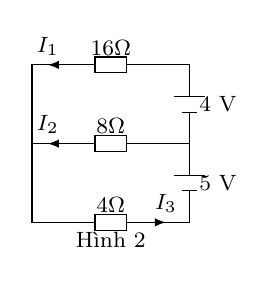
\begin{tikzpicture}
		\tikzset{
			every node/.style={font=\footnotesize,transform shape},
			%
			ampe/.pic={\draw (0,0)circle(0.25) (0,0)node[align=center]{A};},
			%
			vol/.pic={\draw (0,0)circle(0.2) (0,0)node[align=center]{V};},
			% Điện tro
			dientro2/.pic={\draw (-.1,-.2)--(-.1,.2)--(.1,.2)--(.1,-.2)--cycle %(0,0)node[align=center]{Hình\\chữ nhật}
				;},
			% Điện tro
			dientro/.pic={\draw (-.2,-.1)--(-.2,.1)--(.2,.1)--(.2,-.1)--cycle %(0,0)node[align=center]{Hình\\chữ nhật}
				;},
			% Điện tro
			dientro1/.pic={\draw (-.2,-.1)--(-.2,.1)--(.2,.1)--(.2,-.1)--cycle %(0,0)node[align=center]{Hình\\chữ nhật}
				;},
		% nguồn điện
		nguondien1/.pic={\draw  (-.1,-.1)--(.1,-.1) (-.2,.1)--(.2,.1)
			%(0,0)node[align=center]{Hình\\chữ nhật}
			;},
	% nguồn điện
nguondien2/.pic={\draw  (-.1,-.1)--(.1,-.1) (-.2,.1)--(.2,.1)
	%(0,0)node[align=center]{Hình\\chữ nhật}
	;},
			% Điện tro
			dientro3/.pic={\draw (-.2,-.1)--(-.2,.1)--(.2,.1)--(.2,-.1)--cycle %(0,0)node[align=center]{Hình\\chữ nhật}
				;},
		}
		%
		\draw

	%	(2,-.5)pic[local bounding box =dt3]{dientro3}
		(0,2)pic[local bounding box =dt]{dientro}
		(0,1)pic[local bounding box =dt1]{dientro1}
	(0,0)pic[local bounding box =dt3]{dientro3}
		(1,.5)pic[local bounding box =nd1]{nguondien1}
(1,1.5)pic[local bounding box =nd2]{nguondien1}
		;
		%
	\draw[](dt3)node[above]{$4\Omega$}--(1,0)--(nd1)node[right]{ $5$ V}--(nd2)node[right]{ $4$ V}--(1,2)--(dt)node[above]{$16\Omega$}--(-1,2)--(-1,0)--(dt3) (-1,1)--(dt1)node[above]{$8\Omega$}--(1,1);
		\draw[-latex](-0.5,2)--(-0.8,2)node[above]{$I_1$};
		\draw[-latex](-.5,1)--(-0.8,1)node[above]{$I_2$};
		\draw[-latex](0.5,0)--(0.7,0)node[above]{$I_3$};
		%\draw[-latex](0.5,-.5)--(1,-.5)node[above]{$I_5$};
		\draw(0,0)node[below]{Hình 2};
	%	\draw(nd)--(dt1);
\end{tikzpicture}}
	\loigiai{
	Theo đề bài, ta có hệ phương trình: $\left\{\begin{array}{l}I_1+I_2=I_3 \\ 16 I_1-8 I_2=4 \\ 8 I_2+4 I_3=5.\end{array}\right.$\\
	Giải hệ phương trình, ta được: $I_1=\dfrac{11}{28} \mathrm{~A}$; $I_2=\dfrac{2}{7} \mathrm{~A}$; $I_3=\dfrac{19}{28} \mathrm{~A}$.}
	\end{bt}
\begin{bt}%[0D3B3-5]
	Để mở rộng sản suất, một công ty đã vay $800$ triệu đồng từ ba ngân hàng $A, B$ và $C$, với lãi suất cho vay theo năm lần lượt là $6 \%, 8 \%$ và $9 \%$. Biết rằng tổng số tiền lãi năm đầu tiên công ty phải trả cho ba ngân hàng là $60$ triệu đồng và số tiền lãi công ty trả cho hai ngân hàng $A$ và $C$ là bằng nhau. Tính số tiền công ty đã vay từ mỗi ngân hàng.
	\loigiai{
	Gọi $x$, $y$, $z$ lần lượt là số tiền công ty đã vay từ các ngân hàng $A$, $B$, $C$ (đơn vị: triệu đồng, $x \geq 0$, $y \geq 0$, $z \geq 0$).\\
	Theo đề bài, ta có hệ phương trình $\left\{\begin{array}{l}x+y+z=800 \\ 0{,}06 x+0{,}08 y+0{,}09 z=60 \\ 0{,}06 x=0{,}09 z.\end{array}\right.$\\
	Giải hệ phương trình, ta được $x=300$, $y=300$, $z=200$.\\
	Vậy số tiền công ty đã vay từ ba ngân hàng $A$, $B$, $C$ lần lượt là $300$ triệu đồng, $300$ triệu đồng, $200$ triệu đồng.
}
	\end{bt}
\begin{bt}%[0D3B3-5]
	Bác Nhân có $650$ triệu đồng dự định gửi tiết kiệm vào các ngân hàng $A$, $B$ và $C$. Biết các ngân hàng $A$, $B$, $C$ trả lãi suất lần lượt là $8 \% /$năm, $7{,}5 \% /$năm và $7 \% /$năm. Để phù hợp với nhu cầu, bác Nhân mong muốn sau một năm, tồng số tiền lãi bác nhận được là $50$ triệu đồng và số tiền bác gửi vào ngân hàng $B$ lớn hơn số tiền gửi vào ngân hàng $C$ là $100$ triệu đồng. Hãy tính giúp bác Nhân số tiền gửi vào mỗi ngân hàng sao cho đáp ứng được yêu cầu của bác.
	\loigiai{Gọi $x$, $y$, $z$ lần lượt là số tiền bác Nhân đã gửi vào các ngân hàng $A$, $B$, $C$ (đơn vị: triệu đồng, $x \geq 0, y \geq 0, z \geq 0$ ).\\
		Theo bài ra, ta có hệ phương trình $\heva{&x+y+z=650 \\ &0{,}08 x+0{,}075 y+0{,}07 z=50 \\ &y-z=100 .}$\\
		Giải hệ phương trình, ta được $x=350$, $y=200$, $z=100$.\\
		Vậy số tiền nên gưii vào các ngân hàng $A$, $B$, $C$ lần lượt là $350$ triệu đồng, $200$ triệu đồng, $100$ triệu đồng.
	}
		\end{bt}
\begin{bt}%[0D3B3-5]
	Một công ty sản xuất ba loại phân bón:\begin{itemize}
	\item Loại $\mathrm{A}$ có chứa $18 \%$ nitơ, $4 \%$ photphat và $5 \%$ kali;
	\item Loại $\mathrm{B}$ có chứa $20 \%$ nitơ, $4 \%$ photphat và $4 \%$ kali;
	\item Loại $\mathrm{C}$ có chứa $24 \%$ nitơ, $3 \%$ photphat và $6 \%$ kali.
	\end{itemize}
	Công ty sản xuất bao nhiêu kilôgam mỗi loại phân bón trên? Biết rằng công ty đã dùng hết $26400 \mathrm{~kg}$ nitơ, $4900 \mathrm{~kg}$ photphat, $6200 \mathrm{~kg}$ kali.
	\loigiai{
	Gọi $x, y, z$ lần lượt là số kilôgam mỗi loại phân bón $A, B, C$ mà công ty đã sản xuất $(x \geq 0$, $y \geq 0$, $z \geq 0)$.\\
	Theo đề bài, ta có hệ phương trình $\left\{\begin{array}{l}0{,}18 x+0{,}2 y+0{,}24 z=26400 \\ 0{,}04 x+0{,}04 y+0{,}03 z=4900 \\ 0{,}05 x+0{,}04 y+0{,}06 z=6200.\end{array}\right.$\\
	Giải hệ phương trinh, ta được $x=40000$, $y=60000$, $z=30000$.\\
	Vậy khối lượng mỗi loại phân bón $A$, $B$, $C$ mà công ty đã sản xuất lần lượt là $40000 \mathrm{~kg}$, $60000 \mathrm{~kg}$, $30000 \mathrm{~kg}$.
}
	\end{bt}
%KEtNoi
\begin{bt}%[0D3B3-5]
	Cân bằng phương trình phản ứng hoá học đốt cháy octane trong oxygen
	$$
	\mathrm{C}_8 \mathrm{H}_{18}+\mathrm{O}_2 \rightarrow \mathrm{CO}_2+\mathrm{H}_2 \mathrm{O}
	$$
	\loigiai{
	Giả sử $x, y, z, t$ là các số thoả mãn cân bằng
	$$
	x \mathrm{C}_8 \mathrm{H}_{18}+y \mathrm{O}_2 \rightarrow z \mathrm{CO}_2+t \mathrm{H}_2 \mathrm{O} \text {. }
	$$
	Ta có hệ phương trình $\left\{\begin{array}{l}8 x=z \\ 18 x=2 t \\ 2 y=2 z+t.\end{array}\right.$\\
	Giải hệ ta được $z=8 x, t=9 x$ và $y=\dfrac{25}{2} x$.\\
	Chọn $x=2$, được cân bằng
	$$
	2 \mathrm{C}_8 \mathrm{H}_{18}+25 \mathrm{O}_2 \rightarrow 16 \mathrm{CO}_2+18 \mathrm{H}_2 \mathrm{O}.
	$$
}
	\end{bt}
\begin{bt}%[0D3B3-5]
 Xét thị trường hải sản gồm ba mặt hàng là cua, tôm và cá. Kí hiệu $x$, $y$, $z$ lần lượt là giá $1 \mathrm{~kg}$ cua, $1 \mathrm{~kg}$ tôm và $1 \mathrm{~kg}$ cá (đơn vị nghìn đồng). Kí hiệu $Q_{S_1}, Q_{S_2}$ và $Q_{S_3}$ là lượng cua, tôm và cá mà người bán bằng lòng bán với giá $x, y$ và $z$. Kí hiệu $Q_{D_1}$, $Q_{D_2}$ và $Q_{D_3}$ tương ứng là lượng cua, tôm và cá mà người mua bằng lòng mua với giá $x$, $y$ và $z$. Cụ thể các hàm này được cho bởi
	$$
	\begin{aligned}
		&Q_{S_1}=-300+x ; Q_{D_1}=1300-3 x+4 y-z \\
		&Q_{S_2}=-450+3 y ; Q_{D_2}=1150+2 x-5 y-z \\
		&Q_{S_3}=-400+2 z ; Q_{D_3}=900-2 x-3 y+4 z.
	\end{aligned}
	$$
	Tìm mức giá cua, tôm và cá mà người bán và người mua cùng hài lòng.
	\loigiai{
	Hệ phương trình cân bằng cung - cầu $\left\{\begin{array}{l}-300+x=1300-3 x+4 y-z \\ -450+3 y=1150+2 x-5 y-z \\ -400+2 z=900-2 x-3 y+4z.\end{array}\right.$\\
	Giải hệ ta được $x=600, y=300$, $z=400$.\\
	Vậy giá của mỗi kg cua, tôm, cá lần lượt là $600$ nghìn đồng, $300$ nghìn đồng, $400$ nghìn đồng.	
}
	\end{bt}